\documentclass[leqno]{article}
\usepackage[left=0.5in,right=0.5in]{geometry}
\usepackage[utf8]{inputenc}
\usepackage{amsmath, amsfonts, color, booktabs, centernot, graphicx, fancyhdr}
\setlength\parindent{0pt}
\begin{document}
\title{Notes on CS70 Discussion Solutions CrowdSourcing Model}
\author{Leah Dickstein}

\maketitle

\textbf{Current working model:} 
\begin{align*}
grade &= \frac{-time}{efficiency} + knowledge*time + reward * Pr[reward]\\
&= -at + bt + AP[A], 0<a<1 b>1
\end{align*}

\tableofcontents

\section{Experiment 1}
\subsection{Action Plan}
\begin{enumerate}
\item Diagnostic test tells us strength of students
\item Either: 1) Ask how much time it took each student (weaker students should take longer) OR 2) Set a fixed amount of time (weaker students with higher cost will produce lower quality bids) [The way we analyze/compare the following values will vary based on which method was chosen]
\item Calculate relationship between strength and cost
\item Calculate expected bid value
\item Collect actual bid values
\item Compare to theoretical bid value + other variables
\item Calculate expected value
\item Collect actual expected value
\item Compare values
\end{enumerate}

\subsection{Thought Process}
We need to identify:
\begin{itemize}
\item \# of bids is as expected
\item $\mathbb{E} [U]$ as expected
\item Bid values as expected
\end{itemize}

Variables we should know:
\begin{itemize}
\item A -- reward
\item $c_i$ -- cost
\item $x_i$ -- bid
\end{itemize}

\subsubsection*{Need to accomplish:}
1) Rank players by strength to determine their efficiency/knowledge coefficients\\
2) Assign costs: amount of time it takes to complete assignment\\
3) Evaluate bids: Quality of assignment is determined by 1] Correctness 2] Thoroughness (rough estimate = length)\\

\textbf{NOTE:} Need resolution: a regular way to assess student's grades (interpreting that as value/knowledge) for better precision on what activity/event/action corresponded to how large a change in grades

\subsubsection*{1) Strength}
How to rank players by strength:
\begin{enumerate}
\item Ideal: Use Experiment 2's results and control the combination of activities of all the participants
\begin{enumerate}
\item Experiment 2 is supposed to tell you how much each activity matters
\item A student participating in 2 activities should be stronger than a student participating in just 1 (assuming they are equal in everything else, including starting knowledge) so we can rank students that way
\end{enumerate}
\item Baseline diagnostic to assess familiarity with concepts (can be given on first day of class, or as part of Homework 1 along with sign in information)
\item Voluntary poll (can be given on first day of class, Piazza poll looking for voluntary participation) "Which of these concepts/buzzwords have you seen before?"
\end{enumerate}
After that, place data points (students) in bins\\

Assume people stay in bins relative to each other \textcolor{red}{(Not actually true!)}\\
Else: We need regular calibration checks

\subsubsection*{2) Costs}
Need to determine relationship between strength (efficiency/knowledge) and costs:
\begin{enumerate}
\item Ask students how much time they took
\item Only give students a fixed amount of time
\begin{enumerate}
\item Like the practice midterm!
\item For example "There is an extra credit opportunity with no penalty; the only cost is your time."
\item See how many students show up and how they fall in the strength-bins
\end{enumerate}
\item Propose a relationship and see if it's true based on bid values/expected values (e.g. inverse As strength increases costs decrease with some constant factor)
\end{enumerate}

\subsubsection*{3) Bids/Gain}
\begin{itemize}
\item Collect bid values as data points, plot to see relationship with cost/strength/grades
\item If relationship exists, calculate theoretical values of costs, etc. per bin and compare to model
\item Calculate $\mathbb{E} [U_{students}]$, see distribution
\item Check if it matches model
\item How do students' grades change pre $\rightarrow$ post discussion event
\end{itemize}

\section{Experiment 2}
\textbf{Key Point:} Identify how to weight activities, or quantify $\mathbb{E} [value]$ of each activity\\
Later when we're using grades as our measure of value/knowledge, we know what "contribution" is from Discussion Solutions
\subsection{Factors that affect knowledge/grades/expected value}
In no particular order:
\begin{enumerate}
\item Midterm Performance (Required)
\item HW performance (Required)
\item Attendance of HW Parties
\item Attending Lecture
\item Attending Discussion
\item \textcolor{blue}{Doing Discussion problems (submitting solutions)}
\item Having a Study Group
\item Going to Office Hours
\item Reading Lecture Notes
\item Posting Qs/Receiving Feedback from Piazza
\item[] **Not as important but worth mentioning:**
\item Starting Knowledge
\item Stress from other classes $\rightarrow$ Assume this will be reflected by participation in material
\item[] \quad 12.1 Time spent mulling
\item Enjoyment of material/intuition/being able to pick things up quickly $\rightarrow$ Assume not a problem / uniform
\end{enumerate}

\subsection{Ideal Experiment}
Every single person is uniform: they learn the same way, same speed, same starting knowledge, are taking the same classes and therefore dedicate the same amount of time to CS70.\\

I change which of the above 8 activities (3. -- 10.) the students participate in, then see based on grades which activities are helpful and by how much.\\

There are $\sum_{i=1}^8 {8 \choose i}$ possible subsets of the 8 activities, and I want at least 3 data points per subset (minimum needed to fit a line.) This means I would want a population of at least $3\sum_{i=1}^8 {8 \choose i} = 3*254 = 762$. Although we're not quite there yet, with a CS70 student body of over 600 we might be close enough (over 79\%).

\subsection{Realistic Experiment}
Require students to try everything out in the first 1~2 weeks.
\begin{itemize}
\item See what is more effective based on subsequent attendance (assuming students recognize what is best for them)
\item Have students rate their experiences (assuming they recognize what is better for them)
\end{itemize}

\part*{Recap from 2014-03-30}
\addcontentsline{toc}{part}{Recap from 2014-03-30}
\section{Questions}
What is it about the situation that caused it to match a crowdsourcing model? (What criterion defined it as a crowdsourcing problem?)\\
How can we improve the contest so it better fits the goal of the manager? Let's tweak parameters in controlled experiments and see how and by how much parameters affect the outcomes of the contest. Then, let's design the ideal contest for admin and discussion solutions. Let's also observe how students react to different contests to determine how they are learning and what learning styles best suit them.

\section{Description}
\textbf{Players}: Students\\
\textbf{Incentive}: Extra Credit (\textcolor{red}{Is prize value relatively unknown to students? They don't know HOW much extra credit they get until they bid and win for the first time.})\\
\textbf{Manager}: Professor, GSIs, Readers = admin\\
\textbf{Incentive/Goal for Manager}: Get the right discussion solutions and get maximum number of students to learn by participating \emph{with effort.} A third possible goal is to differentiate who the strongest players are.\\
\textbf{Cost of prize to manager}: Virtually nothing if we consider grade inflation to be minimal, thus Utility = value of function f($\overrightarrow{x}$).\\

\section{Comparison}
\subsection{Differences with Gireeja's model}
\begin{enumerate}
\item Players do NOT know each other's strengths
\begin{itemize}
\item However, based on their grades, they know relatively where they are in the class
\item Since it's Berkeley/maybe people in general, many players assume they are "bad" compared to everyone else (\textcolor{red}{assumption??})
\end{itemize}
\item In model, there was a Nash equilibrium where only 2 players bid. Players 3 through n of less strength bid 0 with probability 1. In the current setting 3 people get extra credit, so there should be 3 to 4 players who bid.
\end{enumerate}

\subsection{Connection to Gireeja's paper}
The task is a combination of a selective task and market creation. It's selective because there's a "right" answer to solutions. Even if students post different ways of approaching the problem, there's still a "correct end goal." It's market creation because the managers want as many people to participate as possible with effort, so the more students that participate the better.\\

For selective task, $U_task = max(x_1,x_2,\dots x_n) - A$
\[ \mathbb{E}[U_task] = \frac{A}{6}\left(\frac{3c_2+c_1}{c_2^2}\right) - A \]
This expected utility is positive iff $\frac{3c_2-c_1}{6c_2^2} - 1 > 0$\\
If $c_2 \gg c_1$ then $c_2 < \frac{1}{2}$\\
If $3c_2-c_1 = \epsilon$ is small (low difference) then $c_2^2 < \frac{\epsilon}{6}$ ensures positive utility\\
This is based on $c_1 < c_2$\\

For market creation, $f(\overrightarrow{x}) = \alpha n + \beta$\\
Manager utility doesn't depend on utility of players at all

\subsection{What this means}
If the managers gave everyone extra credit simply for participating, everyone would only put in the minimal bid. This is why the manager wants participation \emph{with effort.} The manager wants to challenge everyone.\\

Since there are elements of both selective task and market creation in the Discussion Solutions situation, we need to decide which one is weighted more and/or how to combine the two to create a model for this scenario.

\section{Data: Updated to 11B}

\subsection{Discussion Solutions}
\begin{tabular}{c c l}
Discussion & \# of bids & Players\\
1B & 4 bids & Hansong Zhang, Kevin Chen, Daniel Suryakusuma, Andrew Luo\\
2A & 5 bids & Viraj Mahesh, Lingtian Cheng, Hansong Zhang, Hongling Lu, Arnav Dugar\\
2B & 5 bids & Lingtian Cheng, Hongling Lu, Melanie Cebula, Myra Haqqi, Arnav Dugar\\
3A & 5 bids & Hongling Lu, Viraj Mahesh, Brian Chu, Myra Haqqi, Arnav Dugar\\
3B & 4 bids & Chris Dock, Hansong Zhang, Hongling Lu, Myra Haqqi\\
4A & 4 bids & Kevin Mawhorter, Hongling Lu, Melanie Cebula, Cong Chen\\
4B & 5 bids & Arnav Dugar, Anurag Ajay, Myra Haqqi, Hongling Lu, Lingtian Cheng\\
5A & 0 bids & Midterm so no solution thread posted\\
5B & 6 bids & Hongling Lu, Arnav Dugar, Aditya Challa, Anurag Ajay, Myra Haqqi, Alex Yang\\
6A & 4 bids & Arnav Dugar, Hongling Lu, Myra Haqqi, Aditya Challa\\
6B & 4 bids & Aditya Challa, Myra Haqqi, Anurag Ajay, Arnav Dugar\\
7A & 4 bids & Aditya Challa, Jong Yun Lee, Myra Haqqi, Max Kanwal\\
7B & 3 bids & Aditya Challa, Max Kanwal, Myra Haqqi\\
8A & 3 bids & Myra Haqqi, Aditya Challa, Liuxiao Zhang\\
8B & 0 bids & Midterm so no solution thread posted\\
9A & 5 bids & Albert Lin, Derek Ahmed, Aditya Challa, Myra Haqqi, Max Kanwal\\
9B & 4 bids & Derek Ahmed, Albert Lin, Aditya Challa, Myra Haqqi\\
10A & 11 bids & Paul Bramsen, Adithyavairavan Murali, Max Kanwal, Josh Zarrabi, Tony Chen, Aditya Challa, Claire Watanabe, Tricia Fu, Derek Ahmed, Yang Rui, Myra Haqqi\\
10B & 5 bids & Janet Chu, Aditya Challa, Yang Rui, Myra Haqqi, Max Kanwal\\
11A & 4 bids & Janet Chu, Aditya Challa, Myra Haqqi, Max Kanwal\\
11B & 2 bids & Aditya Challa, Myra Haqqi
\end{tabular}\\

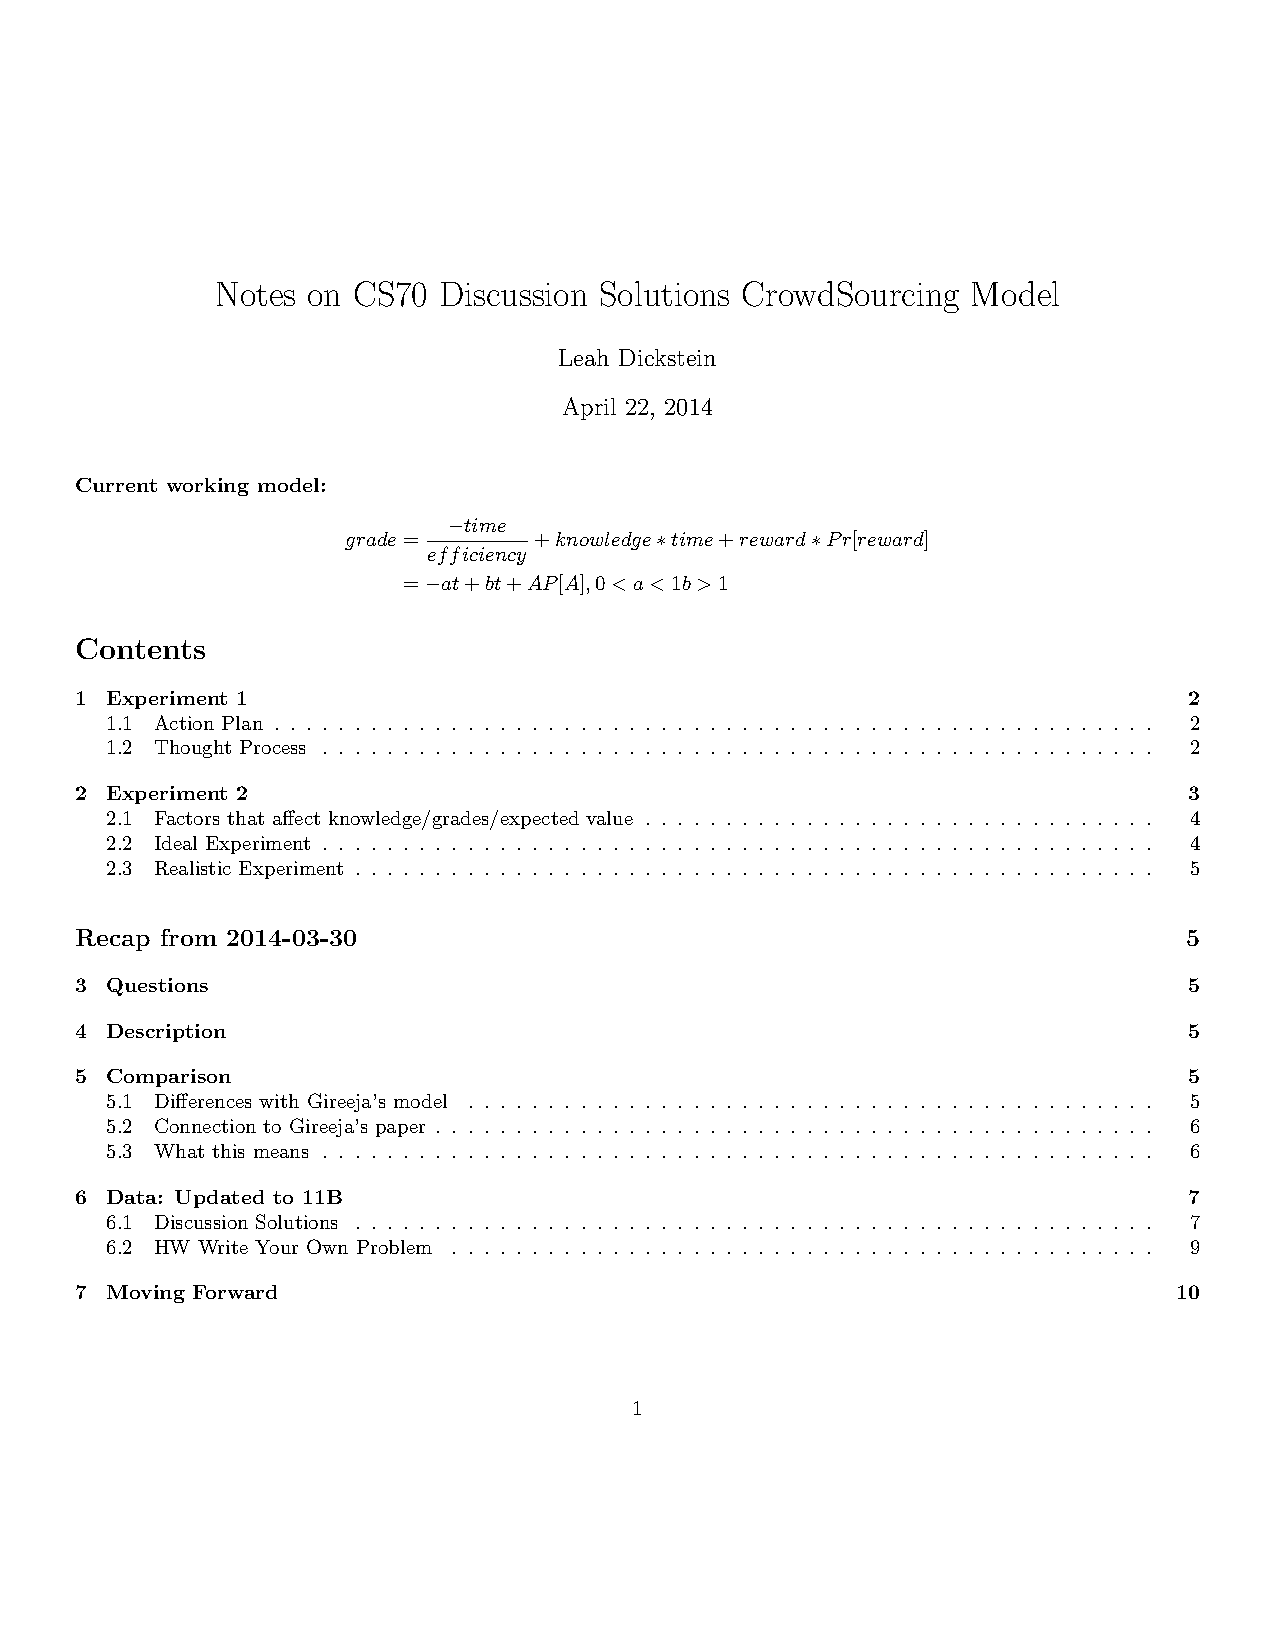
\includegraphics[scale=0.5]{140421}\\

\begin{verbatim}
data = [4, 5, 5, 5, 4, 4, 5, 6, 4, 4, 4, 3, 3, 5, 4, 11, 5, 4, 2];
plot(data)
grid on
set(gca,'xtick',1:19);
ylim([0 11])
set(gca,'XTickLabel',{'1B','2A','2B','3A','3B','4A','4B','5B','6A','6B','7A','7B','8A','9A','9B','10A','10B','11A','11B'})
title('Discussion Solutions Bids 1B-11B')
\end{verbatim}

\textbf{Average bids per contest}: $4\frac{4}{7}$\\

\begin{tabular}{c c}
\# of bids & Frequency\\
2 & 1\\
3 & 2\\
4 & 8\\
5 & 6\\
6 & 1\\
11 & 1\\
\end{tabular}

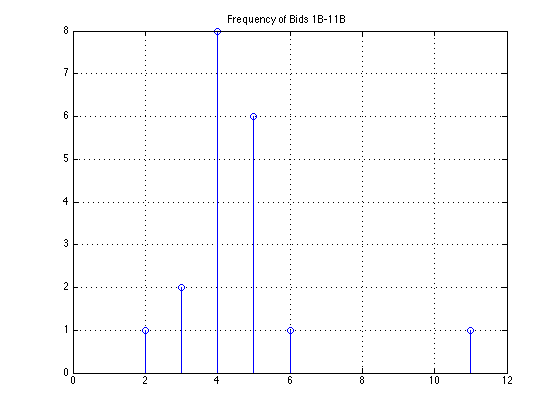
\includegraphics[scale=0.5]{140421_2}\\

The below is updated to 11A.\\

\begin{tabular}{l c l}
Player & \# of bids & Bid dates\\
Aditya Challa & 10 & 5B, 6A, 6B, 7A, 7B, 8A, 9A, 9B, 10A, 10B\\
Adithyavairavan Murali & 1 & 10A\\
Albert Lin & 2 & 9A, 9B\\
Alex Yang & 1 & 5B\\
Andrew Luo & 1 & 1B\\
Anurag Ajay & 3 & 4B, 5B, 6B\\
Arnav Dugar & 7 & 2A, 2B, 3A, 4B, 5B, 6A, 6B\\
Brian Chu & 1 & 3A\\
Chris Dock & 1 & 3B\\
Claire Watanabe & 1 & 10A\\
Cong Chen & 1 & 4A\\
Daniel Suryakusuma & 1 & 1B\\
Derek Ahmed & 3 & 9A, 9B, 10A\\
Hansong Zhang & 3 & 1B, 2A, 3B\\
Hongling Lu & 8 & 2A, 2B, 3A, 3B, 4A, 4B, 5B, 6A\\
Janet Chu & 1 & 10B\\
Jong Yun Lee & 1 & 7A\\
Josh Zarrabi & 1 & 10A\\
Kevin Chen & 1 & 1B\\
Kevin Mawhorter & 1 & 4A\\
Lingtian Cheng & 3 & 2A, 2B, 4B\\
Liuxiao Zhang & 1 & 8A\\
Max Kanwal & 5 & 7A, 7B, 9A, 10A, 10B\\
Melanie Cebula & 2 & 2B, 4A\\
Myra Haqqi & 14 & 2B, 3A, 3B, 4B, 5B, 6A, 6B, 7A, 7B, 8A, 9A, 9B, 10A, 10B\\
Paul Bramsen & 1 & 10A\\
Tony Chen & 1 & 10A\\
Tricia Fu & 1 & 10A\\
Viraj Mahesh & 2 & 2A, 3A\\
Yang Rui & 1 & 10A
\end{tabular}\\

Average bids per player: 2.7\\
After removing the 4 outliers: 1.577\\
Total bid opportunities (contests): 18\\
Total players: 30\\
Returning players $>$ 1 instance: 12 = a little under half!\\

\subsection{HW Write Your Own Problem}
In this case, students have already been forced to bid. Thus, posting online comes only at the cost of going online. There is potential cost in making a good problem while writing HW.\\

\begin{tabular}{c c}
HW \# & \# of Bids\\
2 & 23\\
3 & 11\\
4 & 4\\
5 & 9\\
6 & 7\\
7 & 1\\
8 & 7\\
9 & 7\\
10 & 4\\
11 & 6
\end{tabular}\\

Average number of bids per HW: 7.9\\

These results indicate the majority of the class aren't submitting their own problems. In addition, the difficulty of the problems being submitted appears to have decreased, although I haven't examined them carefully. That could just be hindsight bias.

\section{Moving Forward}
\begin{enumerate}
\item Design ideal experiment for Leah
\item Make ideal experiment realistic
\item Compare already submitted solutions to see how they're chosen for reward and how that relates to bid value/the other variables
\end{enumerate}
\end{document}